%%Initial Setup
%%  A simple AAU report template.
%  2014-09-13 v. 1.1.0
%  Copyright 2010-2014 by Jesper Kjær Nielsen <jkn@es.aau.dk>
%
%  This is free software: you can redistribute it and/or modify
%  it under the terms of the GNU General Public License as published by
%  the Free Software Foundation, either version 3 of the License, or
%  (at your option) any later version.
%
%  This is distributed in the hope that it will be useful,
%  but WITHOUT ANY WARRANTY; without even the implied warranty of
%  MERCHANTABILITY or FITNESS FOR A PARTICULAR PURPOSE.  See the
%  GNU General Public License for more details.
%
%  You can find the GNU General Public License at <http://www.gnu.org/licenses/>.
%
% \documentclass[12pt,twoside,a4paper,openright]{report}
\documentclass[12pt,twoside,a4paper,openany]{report}
%%%%%%%%%%%%%%%%%%%%%%%%%%%%%%%%%%%%%%%%%%%%%%%%
% Language, Encoding and Fonts
% http://en.wikibooks.org/wiki/LaTeX/Internationalization
%%%%%%%%%%%%%%%%%%%%%%%%%%%%%%%%%%%%%%%%%%%%%%%%
% Select encoding of your inputs. Depends on
% your operating system and its default input
% encoding. Typically, you should use
%   Linux  : utf8 (most modern Linux distributions)
%            latin1 
%   Windows: ansinew
%            latin1 (works in most cases)
%   Mac    : applemac
% Notice that you can manually change the input
% encoding of your files by selecting "save as"
% an select the desired input encoding. 
\usepackage[utf8]{inputenc}
% Make latex understand and use the typographic
% rules of the language used in the document.
\usepackage[danish,english]{babel}

%% ssary things
%\usepackage[acronym]{glossaries}
%\makeglossaries




% Use the palatino font
\usepackage[sc]{mathpazo}
\linespread{1.05}         % Palatino needs more leading (space between lines)
% Choose the font encoding
\usepackage[T1]{fontenc}
%%%%%%%%%%%%%%%%%%%%%%%%%%%%%%%%%%%%%%%%%%%%%%%%
% Graphics and Tables
% http://en.wikibooks.org/wiki/LaTeX/Importing_Graphics
% http://en.wikibooks.org/wiki/LaTeX/Tables
% http://en.wikibooks.org/wiki/LaTeX/Colors
%%%%%%%%%%%%%%%%%%%%%%%%%%%%%%%%%%%%%%%%%%%%%%%%
% load a colour package
%%TEMP REMOVED!!!!!!!%%%%%\usepackage{xcolor}
\usepackage[pdftex,dvipsnames]{xcolor}
\definecolor{aaublue}{RGB}{33,26,82}% dark blue
% The standard graphics inclusion package
\usepackage{graphicx}
\graphicspath{{Pictures/}}
% Set up how figure and table captions are displayed
\usepackage{caption}
\captionsetup{%
  font=footnotesize,% set font size to footnotesize
  labelfont=bf % bold label (e.g., Figure 3.2) font
}
\usepackage{subcaption}
% Make the standard latex tables look so much better
\usepackage{array,booktabs}
% Enable the use of frames around, e.g., theorems
% The framed package is used in the example environment
\usepackage{framed}

%%%%%%%%%%%%%%%%%%%%%%%%%%%%%%%%%%%%%%%%%%%%%%%%
% Mathematics
% http://en.wikibooks.org/wiki/LaTeX/Mathematics
%%%%%%%%%%%%%%%%%%%%%%%%%%%%%%%%%%%%%%%%%%%%%%%%
% Defines new environments such as equation,
% align and split 
\usepackage{amsmath}
% Adds new math symbols
\usepackage{amssymb}
% Use theorems in your document
% The ntheorem package is also used for the example environment
% When using thmmarks, amsmath must be an option as well. Otherwise \eqref doesn't work anymore.
\usepackage[framed,amsmath,thmmarks]{ntheorem}

%%%%%%%%%%%%%%%%%%%%%%%%%%%%%%%%%%%%%%%%%%%%%%%%
% Page Layout
% http://en.wikibooks.org/wiki/LaTeX/Page_Layout
%%%%%%%%%%%%%%%%%%%%%%%%%%%%%%%%%%%%%%%%%%%%%%%%
% Change margins, papersize, etc of the document
\usepackage[
	left=15mm,
	right=15mm,
	top=2cm,
	bottom=3cm
	%left=15mm,
	%right=15mm,
	%top=3cm,
	%bottom=3cm
	]{geometry} 
% Modify how \chapter, \section, etc. look
% The titlesec package is very configureable
\usepackage{titlesec}
%\titleformat{\chapter}[display]{\normalfont\huge\bfseries\color{aaublue}}{\chaptertitlename\ \thechapter}{20pt}{\Huge}
\titleformat*{\section}{\normalfont\Large\bfseries\color{aaublue}}
\titleformat*{\subsection}{\normalfont\large\bfseries\color{aaublue}}
\titleformat*{\subsubsection}{\normalfont\normalsize\bfseries\color{aaublue}}
%\titleformat*{\paragraph}{\normalfont\normalsize\bfseries\color{aaublue}}
%\titleformat*{\subparagraph}{\normalfont\normalsize\bfseries\color{aaublue}}

% Clear empty pages between chapters
\let\origdoublepage\cleardoublepage
\newcommand{\clearemptydoublepage}{%
  \clearpage
  {\pagestyle{empty}\origdoublepage}%
}
\let\cleardoublepage\clearemptydoublepage
% Tools to flip page content (tables, pictures, etc.)
\usepackage{adjustbox}
\usepackage{rotating}
% Adjustable table width/height structure
\usepackage{tabularx}
\usepackage[vlines]{tabularht}
% Change the headers and footers
\usepackage{fancyhdr}
\pagestyle{fancy}
\usepackage[Sonny]{fncychap}
\fancyhf{} %delete everything
\renewcommand{\headrulewidth}{0pt} %remove the horizontal line in the header
\fancyhead[RE]{\color{aaublue}\small\nouppercase\leftmark} %even page - chapter title
\fancyhead[LO]{\color{aaublue}\small\nouppercase\rightmark} %uneven page - section title
\fancyhead[LE,RO]{\thepage} %page number on all pages
\setlength{\headheight}{14.5pt} 
% Do not stretch the content of a page. Instead,
% insert white space at the bottom of the page
\raggedbottom
% Enable arithmetics with length. Useful when
% typesetting the layout.
\usepackage{calc}

%%%%%%%%%%%%%%%%%%%%%%%%%%%%%%%%%%%%%%%%%%%%%%%%
% Bibliography
% http://en.wikibooks.org/wiki/LaTeX/Bibliography_Management
%%%%%%%%%%%%%%%%%%%%%%%%%%%%%%%%%%%%%%%%%%%%%%%%
% Add the \citep{key} command which display a
% reference as [author, year]
\usepackage[numbers]{natbib}
% Appearance of the bibliography
\bibliographystyle{plainnat}

%%%%%%%%%%%%%%%%%%%%%%%%%%%%%%%%%%%%%%%%%%%%%%%%
% Misc
%%%%%%%%%%%%%%%%%%%%%%%%%%%%%%%%%%%%%%%%%%%%%%%%
% Include full pdf pages
\usepackage{pdfpages}
% Add bibliography and index to the table of
% contents
\usepackage[nottoc]{tocbibind}
% Add the command \pageref{LastPage} which refers to the
% page number of the last page
\usepackage{lastpage}
% Add todo notes in the margin of the document
\usepackage[
%  disable, %turn off todonotes
colorinlistoftodos, %enable a coloured square in the list of todos
textwidth=\marginparwidth, %set the width of the todonotes
%textsize=scriptsize, %size of the text in the todonotes
]{todonotes}

%%%%%%%%%%%%%%%%%%%%%%%%%%%%%%%%%%%%%%%%%%%%%%%%
% Hyperlinks
% http://en.wikibooks.org/wiki/LaTeX/Hyperlinks
%%%%%%%%%%%%%%%%%%%%%%%%%%%%%%%%%%%%%%%%%%%%%%%%
% Enable hyperlinks and insert info into the pdf
% file. Hypperref should be loaded as one of the 
% last packages
\usepackage{hyperref}
\hypersetup{%
	%pdfpagelabels=true,%
	plainpages=false,%
	pdfauthor={Livia Elena Anghel, Raul Cos, Felix Gravila, Vojtech Jindra, Valer Orlovsky, Miroslav Pakanec},%
	pdftitle={Passenger Classification},%
	pdfsubject={Passenger Classification},%
	pdfkeywords={AAU project 7 semester Passenger Classification Blip System},%
	bookmarksnumbered=true,%
	colorlinks,%
	citecolor=aaublue,%
	filecolor=aaublue,%
	linkcolor=aaublue,% you should probably change this to black before printing
	urlcolor=aaublue,%
	pdfstartview=FitH%
}
\newenvironment{itquote}
  {\begin{quote}\itshape}
  {\end{quote}\ignorespacesafterend}
\usepackage{listings}
\usepackage{float}
\usepackage{wrapfig}
%\usepackage{subfig}
\usepackage{url}

%%\usepackage{minted}
%\definecolor{graa}{rgb}{0.9, 0.9, 0.9}
%\usepackage{tcolorbox}
%\tcbuselibrary{minted,skins}
%\newtcblisting{mintedboks}[1]{
%	listing engine=minted,
%	colback=graa,
%	colframe=black!70,
%	listing only,
%	minted style=colorful,
%	minted language=#1,
%	minted options={
%	    linenos=true,
%	    tabsize=4,
%        texcl=true,
%		fontsize=\footnotesize,
%		numbersep=3mm,
%		breaklines=true,
%		fontfamily=tt
%	},
%	top=-0.5mm,
%	bottom=-0.5mm,
%	left=5mm,
%	enhanced,
%	overlay={\begin{tcbclipinterior}\fill[black!25] (frame.south west)
%	  		rectangle ([xshift=5mm]frame.north west);\end{tcbclipinterior}}
%}

\expandafter\def\expandafter\UrlBreaks\expandafter{\UrlBreaks%  save the current one
  \do\a\do\b\do\c\do\d\do\e\do\f\do\g\do\h\do\i\do\j%
  \do\k\do\l\do\m\do\n\do\o\do\p\do\q\do\r\do\s\do\t%
  \do\u\do\v\do\w\do\x\do\y\do\z\do\A\do\B\do\C\do\D%
  \do\E\do\F\do\G\do\H\do\I\do\J\do\K\do\L\do\M\do\N%
  \do\O\do\P\do\Q\do\R\do\S\do\T\do\U\do\V\do\W\do\X%
  \do\Y\do\Z}

%No indent  
\newlength\tindent
\setlength{\tindent}{\parindent}
\setlength{\parindent}{0pt}
\renewcommand{\indent}{\hspace*{\tindent}}

%\usepackage{etoolbox}
%\makeatletter
%\patchcmd{\FV@SaveLineBox}{%
%	\strut#1\strut
%}{%
%\hyphenchar\font=%
%% Invisible hyphen:
%\if\expandafter\@car\f@encoding\relax\@nil O 255 \else 23 \fi
%% Visible hyphen:
%% `\- %
%\strut
%\nobreak % prevent line break by next \hspace
%\hspace{0pt}% allow hyphenation of first word
%#1%
%\nobreak % without the following \strut would prevent hyphenation of previous word
%\strut
%}{}{%
%\errmessage{\noexpand\FV@SaveLineBox could not be patched}%
%}
\makeatother
\usepackage[linesnumbered]{algorithm2e}
%\usepackage{msctexen}
\usepackage{color}

\usepackage[footnote,draft,silent,nomargin]{fixme}
\fxsetup{theme=color}
%\definecolor{fxtarget}{rgb}{255,0.0000,0.0000}

%Use cleverref
\usepackage[english]{cleveref}

%include eps file extensions
\usepackage{epstopdf}
\epstopdfsetup{outdir=./epsfigs/}

% Forskellige muligheder for todo's
\newcommand{\unsure}[1]{\todo[linecolor=red,backgroundcolor=red!25,bordercolor=red,inline]{LÆS! #1}\mbox{}}
\newcommand{\change}[2][1=]{\todo[linecolor=yellow,backgroundcolor=yellow!25,bordercolor=yellow,#1]{#2}}
\newcommand{\info}[1]{\todo[linecolor=blue,backgroundcolor=blue!25,bordercolor=blue,inline]{#1}}
\newcommand{\missingref}[1]{\todo[linecolor=Magenta,backgroundcolor=Magenta!25,bordercolor=Magenta]{\textbf{Mangler ref!} #1}}
\newcommand{\missingcite}[1]{\todo[linecolor=Magenta,backgroundcolor=Magenta!25,bordercolor=Magenta]{\textbf{Mangler kilde!} #1}}
\newcommand{\missingdesc}[1]{\todo[linecolor=Magenta,backgroundcolor=Magenta!25,bordercolor=Magenta]{\textbf{Mangler beskrivelse!} #1}}

% Sætter hvor mange tal der skal gives ud og hvor mange der skal vises i indholdsfortegnelse
\setcounter{tocdepth}{2}
\setcounter{secnumdepth}{2}

%
\setlength{\emergencystretch}{3em}
\renewcommand{\bibfont}{\footnotesize}

\newcommand{\specialcell}[2][c]{%
  \begin{tabular}[#1]{@{}L@{}}#2\end{tabular}}
\newcommand{\specialcellTen}[2][c]{%
  \begin{tabular}[#1]{@{}L{10cm}@{}}#2\end{tabular}}
  
\usepackage{array}
\newcolumntype{L}[1]{>{\raggedright\let\newline\\\arraybackslash\hspace{0pt}}m{#1}}
\newcolumntype{C}[1]{>{\centering\let\newline\\\arraybackslash\hspace{0pt}}m{#1}}
\newcolumntype{R}[1]{>{\raggedleft\let\newline\\\arraybackslash\hspace{0pt}}m{#1}}
%\usepackage{tabularx}
\usepackage{ltablex}

%\usepackage[acronym,shortcuts,acronymlists={hidden},nonumberlist]{glossaries} % If no numbers are wanted nonumberlist
%
%\newglossary[algh]{hidden}{acrh}{acnh}{Hidden Acronyms}
%%\makeglossaries
%\makenoidxglossaries


%make examplesss!!!
\newtheorem{example}{Example}

\usepackage{multirow}

%% see, e.g., http://en.wikibooks.org/wiki/LaTeX/Formatting#Hyphenation
% for more information on word hyphenation
\hyphenation{ex-am-ple hy-phen-a-tion short}
\hyphenation{long la-tex}

%%  A simple AAU report template.
%  2015-05-08 v. 1.2.0
%  Copyright 2010-2015 by Jesper Kjær Nielsen <jkn@es.aau.dk>
%
%  This is free software: you can redistribute it and/or modify
%  it under the terms of the GNU General Public License as published by
%  the Free Software Foundation, either version 3 of the License, or
%  (at your option) any later version.
%
%  This is distributed in the hope that it will be useful,
%  but WITHOUT ANY WARRANTY; without even the implied warranty of
%  MERCHANTABILITY or FITNESS FOR A PARTICULAR PURPOSE.  See the
%  GNU General Public License for more details.
%
%  You can find the GNU General Public License at <http://www.gnu.org/licenses/>.
%
%
%
% see, e.g., http://en.wikibooks.org/wiki/LaTeX/Customizing_LaTeX#New_commands
% for more information on how to create macros

%%%%%%%%%%%%%%%%%%%%%%%%%%%%%%%%%%%%%%%%%%%%%%%%
% Macros for the titlepage
%%%%%%%%%%%%%%%%%%%%%%%%%%%%%%%%%%%%%%%%%%%%%%%%
%Creates the aau titlepage
\newcommand{\aautitlepage}[3]{%
	{
		%set up various length
		\ifx\titlepageleftcolumnwidth\undefined
		\newlength{\titlepageleftcolumnwidth}
		\newlength{\titlepagerightcolumnwidth}
		\fi
		\setlength{\titlepageleftcolumnwidth}{0.5\textwidth-\tabcolsep}
		\setlength{\titlepagerightcolumnwidth}{\textwidth-2\tabcolsep-\titlepageleftcolumnwidth}
		%create title page
		\thispagestyle{empty}
		\noindent%
		\begin{tabular}{@{}ll@{}}
			\parbox{\titlepageleftcolumnwidth}{
				\iflanguage{danish}{%
					\includegraphics[width=0.75\titlepageleftcolumnwidth]{Pictures/aau_logo_da}
				}{%
				
\includegraphics[width=0.75\titlepageleftcolumnwidth]{Pictures/aau_logo_en}
			}
		} &
		\parbox{\titlepagerightcolumnwidth}{\raggedleft\sf\small
			#2
		}\bigskip\\
		#1 &
		\parbox[t]{\titlepagerightcolumnwidth}{%
			\textbf{Abstract:}\bigskip\par
			\fbox{\parbox{\titlepagerightcolumnwidth-2\fboxsep-2\fboxrule}{%
					#3
				}}
			}\\
		\end{tabular}
		\vfill
		\iflanguage{danish}{%
			\noindent{\footnotesize\emph{Rapportens indhold er frit tilgængeligt, men offentliggørelse (med kildeangivelse) må kun ske efter aftale med forfatterne.}}
		}{%
		\noindent{\footnotesize\emph{The content of this report is freely available, but publication (with reference) may only be pursued due to agreement with the authors.}}
	}
	\clearpage
}
}

%Create english project info
\newcommand{\englishprojectinfo}[7]{%
	\parbox[t]{\titlepageleftcolumnwidth}{
		\textbf{Title:}\\ #1\bigskip\par
		\textbf{Theme:}\\ #2\bigskip\par
		\textbf{Project Period:}\\ #3\bigskip\par
		\textbf{Project Group:}\\ #4\bigskip\par
		\textbf{Participant(s):}\\ #5\bigskip\par
		\textbf{Supervisor(s):}\\ #6\bigskip\par
		\textbf{Page Numbers:} \pageref{LastPage}\bigskip\par
		\textbf{Date of Completion:}\\ #7
	}
}

%Create danish project info
\newcommand{\danishprojectinfo}[8]{%
	\parbox[t]{\titlepageleftcolumnwidth}{
		\textbf{Titel:}\\ #1\bigskip\par
		\textbf{Tema:}\\ #2\bigskip\par
		\textbf{Projektperiode:}\\ #3\bigskip\par
		\textbf{Projektgruppe:}\\ #4\bigskip\par
		\textbf{Deltager(e):}\\ #5\bigskip\par
		\textbf{Vejleder(e):}\\ #6\bigskip\par
		\textbf{Oplagstal:} #7\bigskip\par
		\textbf{Sidetal:} \pageref{LastPage}\bigskip\par
		\textbf{Afleveringsdato:}\\ #8
	}
}

%%%%%%%%%%%%%%%%%%%%%%%%%%%%%%%%%%%%%%%%%%%%%%%%
% An example environment
%%%%%%%%%%%%%%%%%%%%%%%%%%%%%%%%%%%%%%%%%%%%%%%%
\theoremheaderfont{\normalfont\bfseries}
\theorembodyfont{\normalfont}
\theoremstyle{break}
\def\theoremframecommand{{\color{gray!50}\vrule width 5pt \hspace{5pt}}}
\newshadedtheorem{exa}{Example}[chapter]
%\newenvironment{example}[1]{%
%	\begin{exa}[#1]
%	}{%
%\end{exa}
%}

%%\usepackage{glossaries}
%
%%Starting the document
%\begin{document}
%
%%Frontmatter
%\pagenumbering{roman} %use roman page numbering in the frontmatter
%
%\begin{titlepage}
  \noindent%
  \begin{tabular}{@{}p{\textwidth}@{}}
    \toprule[2pt]
    \midrule
    \vspace{0.2cm}
    \begin{center}
    \LARGE{\textbf{
      The Aros Programming Language% insert your title here
    }}
    \end{center}
    %\begin{center}
     % \Large{
      %  - The use of probes to collect mobile wireless data -% insert your subtitle here
     % }
    %\end{center}
    \vspace{0.2cm}\\
    \midrule
    \toprule[2pt]
  \end{tabular}
  \vspace{4 cm}
  \begin{center}
    \vspace{0.2cm}
    {\Large
     P7 Project\\Group d808f19 %Insert your group name or real names here
      \break
      
      
\includegraphics[width=.6\textwidth]{aau_logo_en}
    }
  \end{center}
  \vfill
  \begin{center}
  Aalborg University\\
  Computer Science
  \end{center}
\end{titlepage}
\cleardoublepage
 %Frontpage
%\pdfbookmark[0]{Title page}{label:titlepage_en}
\aautitlepage{%
  \englishprojectinfo{
    Passenger Classification%title
  }{%
	Replacing manual labor of Blip Systems which involve passengers classification in airports%theme
  }{%
    Fall Semester 2018 %project period
  }{%
    Group d705e18 % project group
  }{%
    %list of group members
    \break
    Livia Elena Anghel\\
    \break
    Raul Cos\\
    \break
    Felix Gravila\\
    \break
    Vojtěch Jindra\\
    \break
    Valer Orlovsky\\
    \break
    Miroslav Pakanec\\
   
  }{%
    %list of supervisors
    Chenjuan Guo
  }{%
    \today % date of completion
  }%
}{%department and address
  \textbf{Computer Science}\\
  Aalborg University\\
  \href{http://www.aau.dk}{http://www.aau.dk}
}{% the abstract
This paper describes the modelling and classification of multidimensional time-series with the purpose of classifying different types of individuals observed at an airport, based on wireless sensor readings. Several models were developed to represent the collection of sensor readings for a specific mobile device and used together with machine learning techniques, such as label propagation, decision tree learning and convolutional neural networks. The sparse data set has made it challenging to model differences between individual time-series of mobile devices, which is why a data representation with contextually extracted features was initially favoured and used together with decision trees to achieve a significantly higher accuracy. Finally, the multidimensional time-series representation was revisited and used to train a convolutional neural network in order to automatically detect features, which yielded the best results overall.
}

\cleardoublepage


 %Danish and English title pages
%\chapter*{Preface} \label{sec:forord}
\subsubsection*{Acknowledgements}
We would like to thank our supervisor, Asst. Professor Chenjuan Guo, for the guidance and help she has given us during our project meetings. We would also like to thank BLIP Systems for providing us with the data set and, likewise, Benjamin Krogh for being our contact from BLIP Systems and helping us understand the data.
\bigskip
\begin{flushright}
\textit{Aalborg University, December 20, 2018}
\end{flushright}
\newcommand*\signatureline[2]{\vspace*{2cm}\parbox{5cm}{
    \begin{center}
        \hrulefill\par#1\par#2
    \end{center}
    }
}
\newcommand*\mailto[1]{\href{mailto:#1}{[#1]}}

\begingroup
  \centering
  \signatureline{Livia Elena Anghel}{\mailto{langhe17@student.aau.dk}}
  \hspace{1cm}
  \signatureline{Raul Cos}{\mailto{rcos18@student.aau.dk}}
  \hspace{1cm}
  \signatureline{Felix Gravila}{\mailto{fgravi18@student.aau.dk}}
  \vspace{1cm}
  \signatureline{Vojtěch Jindra}{\mailto{vjindr18@student.aau.dk}}
  \hspace{1cm}
  \signatureline{Valer Orlovsky}{\mailto{vorlov18@student.aau.dk}}
  \hspace{1cm}
  \signatureline{Miroslav Pakanec}{\mailto{mpakan18@student.aau.dk}}
\endgroup

\clearpage
 %Preface
%% \chapter*{Glossary} \label{chap:glossary}

\begin{table}[H]
	\centering
	\begin{tabular}{l|l}
		\toprule
		\textbf{Acronym} & \textbf{Description.} \\ \midrule
		\textbf{AAU} & Aalborg University. \\
		\textbf{C-DB} & Central Database.  \\
		\textbf{GS} & Green Shoots. \\
		\textbf{L-DB} & Local Database. \\
		\textbf{LTE} & Long Term Evolution. \\
		\textbf{OFF-S} & OFF-LINE SCHOOL. \\
		\textbf{ON-S} & ON-LINE SCHOOL. \\
		\bottomrule
	\end{tabular}
\end{table}

%\newglossaryentry{gs}{name=GS, description={Green Shoots}}
%\newglossaryentry{aau}{name=AAU, description={Aalborg University}}
%\newglossaryentry{ofs}{name=OFF-S, description={OFF-LINE SCHOOL}}
%\newglossaryentry{ons}{name=ON-S, description={ON-LINE SCHOOL}}
%\newglossaryentry{lte}{name=LTE, description={Long-Term Evolution}}
%\newglossaryentry{cdb}{name=C-DB, description={Central Database}}
%\newglossaryentry{ldb}{name=L-DB, description={Local Database}}

%\printglossaries

\clearpage %Glossary
%
%%\selectlanguage{danish} %Start specific language
%\pdfbookmark[0]{Contents}{label:contents} %Make PDF bookmarks
%\renewcommand{\contentsname}{Table of contents} %Change table of contents name
%\pagestyle{fancy} %Change page style. Enable headers and footers again
%
%\tableofcontents %Table of contents
%%\addcontentsline{toc}{chapter}{Table of contents}
%%\listoffixmes
%%\listoftodos
%\setcounter{chapter}{0} %Chapter counter
%
%%Mainmatter
%\newpage
%%\printnoidxglossaries %% Printing Glossari page
%
%%\input{Report/introduction.tex}
%%\input{Report/glossary_entry}
%\input{Report/introduction2.tex}
%\input{Report/probAnalysis.tex}
%
%\clearpage
%
%%\pagenumbering{gobble}
%
%%Figurliste
%\listoffigures
%
%%Tabelliste
%\listoftables
%
%%Litteraturliste
%
%%Bilag
%\input{Bilag/bilag.tex}
%
%\end{document}



%Initial Setup
%  A simple AAU report template.
%  2014-09-13 v. 1.1.0
%  Copyright 2010-2014 by Jesper Kjær Nielsen <jkn@es.aau.dk>
%
%  This is free software: you can redistribute it and/or modify
%  it under the terms of the GNU General Public License as published by
%  the Free Software Foundation, either version 3 of the License, or
%  (at your option) any later version.
%
%  This is distributed in the hope that it will be useful,
%  but WITHOUT ANY WARRANTY; without even the implied warranty of
%  MERCHANTABILITY or FITNESS FOR A PARTICULAR PURPOSE.  See the
%  GNU General Public License for more details.
%
%  You can find the GNU General Public License at <http://www.gnu.org/licenses/>.
%
% \documentclass[12pt,twoside,a4paper,openright]{report}
\documentclass[12pt,twoside,a4paper,openany]{report}
%%%%%%%%%%%%%%%%%%%%%%%%%%%%%%%%%%%%%%%%%%%%%%%%
% Language, Encoding and Fonts
% http://en.wikibooks.org/wiki/LaTeX/Internationalization
%%%%%%%%%%%%%%%%%%%%%%%%%%%%%%%%%%%%%%%%%%%%%%%%
% Select encoding of your inputs. Depends on
% your operating system and its default input
% encoding. Typically, you should use
%   Linux  : utf8 (most modern Linux distributions)
%            latin1 
%   Windows: ansinew
%            latin1 (works in most cases)
%   Mac    : applemac
% Notice that you can manually change the input
% encoding of your files by selecting "save as"
% an select the desired input encoding. 
\usepackage[utf8]{inputenc}
% Make latex understand and use the typographic
% rules of the language used in the document.
\usepackage[danish,english]{babel}

%% ssary things
%\usepackage[acronym]{glossaries}
%\makeglossaries




% Use the palatino font
\usepackage[sc]{mathpazo}
\linespread{1.05}         % Palatino needs more leading (space between lines)
% Choose the font encoding
\usepackage[T1]{fontenc}
%%%%%%%%%%%%%%%%%%%%%%%%%%%%%%%%%%%%%%%%%%%%%%%%
% Graphics and Tables
% http://en.wikibooks.org/wiki/LaTeX/Importing_Graphics
% http://en.wikibooks.org/wiki/LaTeX/Tables
% http://en.wikibooks.org/wiki/LaTeX/Colors
%%%%%%%%%%%%%%%%%%%%%%%%%%%%%%%%%%%%%%%%%%%%%%%%
% load a colour package
%%TEMP REMOVED!!!!!!!%%%%%\usepackage{xcolor}
\usepackage[pdftex,dvipsnames]{xcolor}
\definecolor{aaublue}{RGB}{33,26,82}% dark blue
% The standard graphics inclusion package
\usepackage{graphicx}
\graphicspath{{Pictures/}}
% Set up how figure and table captions are displayed
\usepackage{caption}
\captionsetup{%
  font=footnotesize,% set font size to footnotesize
  labelfont=bf % bold label (e.g., Figure 3.2) font
}
\usepackage{subcaption}
% Make the standard latex tables look so much better
\usepackage{array,booktabs}
% Enable the use of frames around, e.g., theorems
% The framed package is used in the example environment
\usepackage{framed}

%%%%%%%%%%%%%%%%%%%%%%%%%%%%%%%%%%%%%%%%%%%%%%%%
% Mathematics
% http://en.wikibooks.org/wiki/LaTeX/Mathematics
%%%%%%%%%%%%%%%%%%%%%%%%%%%%%%%%%%%%%%%%%%%%%%%%
% Defines new environments such as equation,
% align and split 
\usepackage{amsmath}
% Adds new math symbols
\usepackage{amssymb}
% Use theorems in your document
% The ntheorem package is also used for the example environment
% When using thmmarks, amsmath must be an option as well. Otherwise \eqref doesn't work anymore.
\usepackage[framed,amsmath,thmmarks]{ntheorem}

%%%%%%%%%%%%%%%%%%%%%%%%%%%%%%%%%%%%%%%%%%%%%%%%
% Page Layout
% http://en.wikibooks.org/wiki/LaTeX/Page_Layout
%%%%%%%%%%%%%%%%%%%%%%%%%%%%%%%%%%%%%%%%%%%%%%%%
% Change margins, papersize, etc of the document
\usepackage[
	left=15mm,
	right=15mm,
	top=2cm,
	bottom=3cm
	%left=15mm,
	%right=15mm,
	%top=3cm,
	%bottom=3cm
	]{geometry} 
% Modify how \chapter, \section, etc. look
% The titlesec package is very configureable
\usepackage{titlesec}
%\titleformat{\chapter}[display]{\normalfont\huge\bfseries\color{aaublue}}{\chaptertitlename\ \thechapter}{20pt}{\Huge}
\titleformat*{\section}{\normalfont\Large\bfseries\color{aaublue}}
\titleformat*{\subsection}{\normalfont\large\bfseries\color{aaublue}}
\titleformat*{\subsubsection}{\normalfont\normalsize\bfseries\color{aaublue}}
%\titleformat*{\paragraph}{\normalfont\normalsize\bfseries\color{aaublue}}
%\titleformat*{\subparagraph}{\normalfont\normalsize\bfseries\color{aaublue}}

% Clear empty pages between chapters
\let\origdoublepage\cleardoublepage
\newcommand{\clearemptydoublepage}{%
  \clearpage
  {\pagestyle{empty}\origdoublepage}%
}
\let\cleardoublepage\clearemptydoublepage
% Tools to flip page content (tables, pictures, etc.)
\usepackage{adjustbox}
\usepackage{rotating}
% Adjustable table width/height structure
\usepackage{tabularx}
\usepackage[vlines]{tabularht}
% Change the headers and footers
\usepackage{fancyhdr}
\pagestyle{fancy}
\usepackage[Sonny]{fncychap}
\fancyhf{} %delete everything
\renewcommand{\headrulewidth}{0pt} %remove the horizontal line in the header
\fancyhead[RE]{\color{aaublue}\small\nouppercase\leftmark} %even page - chapter title
\fancyhead[LO]{\color{aaublue}\small\nouppercase\rightmark} %uneven page - section title
\fancyhead[LE,RO]{\thepage} %page number on all pages
\setlength{\headheight}{14.5pt} 
% Do not stretch the content of a page. Instead,
% insert white space at the bottom of the page
\raggedbottom
% Enable arithmetics with length. Useful when
% typesetting the layout.
\usepackage{calc}

%%%%%%%%%%%%%%%%%%%%%%%%%%%%%%%%%%%%%%%%%%%%%%%%
% Bibliography
% http://en.wikibooks.org/wiki/LaTeX/Bibliography_Management
%%%%%%%%%%%%%%%%%%%%%%%%%%%%%%%%%%%%%%%%%%%%%%%%
% Add the \citep{key} command which display a
% reference as [author, year]
\usepackage[numbers]{natbib}
% Appearance of the bibliography
\bibliographystyle{plainnat}

%%%%%%%%%%%%%%%%%%%%%%%%%%%%%%%%%%%%%%%%%%%%%%%%
% Misc
%%%%%%%%%%%%%%%%%%%%%%%%%%%%%%%%%%%%%%%%%%%%%%%%
% Include full pdf pages
\usepackage{pdfpages}
% Add bibliography and index to the table of
% contents
\usepackage[nottoc]{tocbibind}
% Add the command \pageref{LastPage} which refers to the
% page number of the last page
\usepackage{lastpage}
% Add todo notes in the margin of the document
\usepackage[
%  disable, %turn off todonotes
colorinlistoftodos, %enable a coloured square in the list of todos
textwidth=\marginparwidth, %set the width of the todonotes
%textsize=scriptsize, %size of the text in the todonotes
]{todonotes}

%%%%%%%%%%%%%%%%%%%%%%%%%%%%%%%%%%%%%%%%%%%%%%%%
% Hyperlinks
% http://en.wikibooks.org/wiki/LaTeX/Hyperlinks
%%%%%%%%%%%%%%%%%%%%%%%%%%%%%%%%%%%%%%%%%%%%%%%%
% Enable hyperlinks and insert info into the pdf
% file. Hypperref should be loaded as one of the 
% last packages
\usepackage{hyperref}
\hypersetup{%
	%pdfpagelabels=true,%
	plainpages=false,%
	pdfauthor={Livia Elena Anghel, Raul Cos, Felix Gravila, Vojtech Jindra, Valer Orlovsky, Miroslav Pakanec},%
	pdftitle={Passenger Classification},%
	pdfsubject={Passenger Classification},%
	pdfkeywords={AAU project 7 semester Passenger Classification Blip System},%
	bookmarksnumbered=true,%
	colorlinks,%
	citecolor=aaublue,%
	filecolor=aaublue,%
	linkcolor=aaublue,% you should probably change this to black before printing
	urlcolor=aaublue,%
	pdfstartview=FitH%
}
\newenvironment{itquote}
  {\begin{quote}\itshape}
  {\end{quote}\ignorespacesafterend}
\usepackage{listings}
\usepackage{float}
\usepackage{wrapfig}
%\usepackage{subfig}
\usepackage{url}

%%\usepackage{minted}
%\definecolor{graa}{rgb}{0.9, 0.9, 0.9}
%\usepackage{tcolorbox}
%\tcbuselibrary{minted,skins}
%\newtcblisting{mintedboks}[1]{
%	listing engine=minted,
%	colback=graa,
%	colframe=black!70,
%	listing only,
%	minted style=colorful,
%	minted language=#1,
%	minted options={
%	    linenos=true,
%	    tabsize=4,
%        texcl=true,
%		fontsize=\footnotesize,
%		numbersep=3mm,
%		breaklines=true,
%		fontfamily=tt
%	},
%	top=-0.5mm,
%	bottom=-0.5mm,
%	left=5mm,
%	enhanced,
%	overlay={\begin{tcbclipinterior}\fill[black!25] (frame.south west)
%	  		rectangle ([xshift=5mm]frame.north west);\end{tcbclipinterior}}
%}

\expandafter\def\expandafter\UrlBreaks\expandafter{\UrlBreaks%  save the current one
  \do\a\do\b\do\c\do\d\do\e\do\f\do\g\do\h\do\i\do\j%
  \do\k\do\l\do\m\do\n\do\o\do\p\do\q\do\r\do\s\do\t%
  \do\u\do\v\do\w\do\x\do\y\do\z\do\A\do\B\do\C\do\D%
  \do\E\do\F\do\G\do\H\do\I\do\J\do\K\do\L\do\M\do\N%
  \do\O\do\P\do\Q\do\R\do\S\do\T\do\U\do\V\do\W\do\X%
  \do\Y\do\Z}

%No indent  
\newlength\tindent
\setlength{\tindent}{\parindent}
\setlength{\parindent}{0pt}
\renewcommand{\indent}{\hspace*{\tindent}}

%\usepackage{etoolbox}
%\makeatletter
%\patchcmd{\FV@SaveLineBox}{%
%	\strut#1\strut
%}{%
%\hyphenchar\font=%
%% Invisible hyphen:
%\if\expandafter\@car\f@encoding\relax\@nil O 255 \else 23 \fi
%% Visible hyphen:
%% `\- %
%\strut
%\nobreak % prevent line break by next \hspace
%\hspace{0pt}% allow hyphenation of first word
%#1%
%\nobreak % without the following \strut would prevent hyphenation of previous word
%\strut
%}{}{%
%\errmessage{\noexpand\FV@SaveLineBox could not be patched}%
%}
\makeatother
\usepackage[linesnumbered]{algorithm2e}
%\usepackage{msctexen}
\usepackage{color}

\usepackage[footnote,draft,silent,nomargin]{fixme}
\fxsetup{theme=color}
%\definecolor{fxtarget}{rgb}{255,0.0000,0.0000}

%Use cleverref
\usepackage[english]{cleveref}

%include eps file extensions
\usepackage{epstopdf}
\epstopdfsetup{outdir=./epsfigs/}

% Forskellige muligheder for todo's
\newcommand{\unsure}[1]{\todo[linecolor=red,backgroundcolor=red!25,bordercolor=red,inline]{LÆS! #1}\mbox{}}
\newcommand{\change}[2][1=]{\todo[linecolor=yellow,backgroundcolor=yellow!25,bordercolor=yellow,#1]{#2}}
\newcommand{\info}[1]{\todo[linecolor=blue,backgroundcolor=blue!25,bordercolor=blue,inline]{#1}}
\newcommand{\missingref}[1]{\todo[linecolor=Magenta,backgroundcolor=Magenta!25,bordercolor=Magenta]{\textbf{Mangler ref!} #1}}
\newcommand{\missingcite}[1]{\todo[linecolor=Magenta,backgroundcolor=Magenta!25,bordercolor=Magenta]{\textbf{Mangler kilde!} #1}}
\newcommand{\missingdesc}[1]{\todo[linecolor=Magenta,backgroundcolor=Magenta!25,bordercolor=Magenta]{\textbf{Mangler beskrivelse!} #1}}

% Sætter hvor mange tal der skal gives ud og hvor mange der skal vises i indholdsfortegnelse
\setcounter{tocdepth}{2}
\setcounter{secnumdepth}{2}

%
\setlength{\emergencystretch}{3em}
\renewcommand{\bibfont}{\footnotesize}

\newcommand{\specialcell}[2][c]{%
  \begin{tabular}[#1]{@{}L@{}}#2\end{tabular}}
\newcommand{\specialcellTen}[2][c]{%
  \begin{tabular}[#1]{@{}L{10cm}@{}}#2\end{tabular}}
  
\usepackage{array}
\newcolumntype{L}[1]{>{\raggedright\let\newline\\\arraybackslash\hspace{0pt}}m{#1}}
\newcolumntype{C}[1]{>{\centering\let\newline\\\arraybackslash\hspace{0pt}}m{#1}}
\newcolumntype{R}[1]{>{\raggedleft\let\newline\\\arraybackslash\hspace{0pt}}m{#1}}
%\usepackage{tabularx}
\usepackage{ltablex}

%\usepackage[acronym,shortcuts,acronymlists={hidden},nonumberlist]{glossaries} % If no numbers are wanted nonumberlist
%
%\newglossary[algh]{hidden}{acrh}{acnh}{Hidden Acronyms}
%%\makeglossaries
%\makenoidxglossaries


%make examplesss!!!
\newtheorem{example}{Example}

\usepackage{multirow}

% see, e.g., http://en.wikibooks.org/wiki/LaTeX/Formatting#Hyphenation
% for more information on word hyphenation
\hyphenation{ex-am-ple hy-phen-a-tion short}
\hyphenation{long la-tex}

%  A simple AAU report template.
%  2015-05-08 v. 1.2.0
%  Copyright 2010-2015 by Jesper Kjær Nielsen <jkn@es.aau.dk>
%
%  This is free software: you can redistribute it and/or modify
%  it under the terms of the GNU General Public License as published by
%  the Free Software Foundation, either version 3 of the License, or
%  (at your option) any later version.
%
%  This is distributed in the hope that it will be useful,
%  but WITHOUT ANY WARRANTY; without even the implied warranty of
%  MERCHANTABILITY or FITNESS FOR A PARTICULAR PURPOSE.  See the
%  GNU General Public License for more details.
%
%  You can find the GNU General Public License at <http://www.gnu.org/licenses/>.
%
%
%
% see, e.g., http://en.wikibooks.org/wiki/LaTeX/Customizing_LaTeX#New_commands
% for more information on how to create macros

%%%%%%%%%%%%%%%%%%%%%%%%%%%%%%%%%%%%%%%%%%%%%%%%
% Macros for the titlepage
%%%%%%%%%%%%%%%%%%%%%%%%%%%%%%%%%%%%%%%%%%%%%%%%
%Creates the aau titlepage
\newcommand{\aautitlepage}[3]{%
	{
		%set up various length
		\ifx\titlepageleftcolumnwidth\undefined
		\newlength{\titlepageleftcolumnwidth}
		\newlength{\titlepagerightcolumnwidth}
		\fi
		\setlength{\titlepageleftcolumnwidth}{0.5\textwidth-\tabcolsep}
		\setlength{\titlepagerightcolumnwidth}{\textwidth-2\tabcolsep-\titlepageleftcolumnwidth}
		%create title page
		\thispagestyle{empty}
		\noindent%
		\begin{tabular}{@{}ll@{}}
			\parbox{\titlepageleftcolumnwidth}{
				\iflanguage{danish}{%
					\includegraphics[width=0.75\titlepageleftcolumnwidth]{Pictures/aau_logo_da}
				}{%
				
\includegraphics[width=0.75\titlepageleftcolumnwidth]{Pictures/aau_logo_en}
			}
		} &
		\parbox{\titlepagerightcolumnwidth}{\raggedleft\sf\small
			#2
		}\bigskip\\
		#1 &
		\parbox[t]{\titlepagerightcolumnwidth}{%
			\textbf{Abstract:}\bigskip\par
			\fbox{\parbox{\titlepagerightcolumnwidth-2\fboxsep-2\fboxrule}{%
					#3
				}}
			}\\
		\end{tabular}
		\vfill
		\iflanguage{danish}{%
			\noindent{\footnotesize\emph{Rapportens indhold er frit tilgængeligt, men offentliggørelse (med kildeangivelse) må kun ske efter aftale med forfatterne.}}
		}{%
		\noindent{\footnotesize\emph{The content of this report is freely available, but publication (with reference) may only be pursued due to agreement with the authors.}}
	}
	\clearpage
}
}

%Create english project info
\newcommand{\englishprojectinfo}[7]{%
	\parbox[t]{\titlepageleftcolumnwidth}{
		\textbf{Title:}\\ #1\bigskip\par
		\textbf{Theme:}\\ #2\bigskip\par
		\textbf{Project Period:}\\ #3\bigskip\par
		\textbf{Project Group:}\\ #4\bigskip\par
		\textbf{Participant(s):}\\ #5\bigskip\par
		\textbf{Supervisor(s):}\\ #6\bigskip\par
		\textbf{Page Numbers:} \pageref{LastPage}\bigskip\par
		\textbf{Date of Completion:}\\ #7
	}
}

%Create danish project info
\newcommand{\danishprojectinfo}[8]{%
	\parbox[t]{\titlepageleftcolumnwidth}{
		\textbf{Titel:}\\ #1\bigskip\par
		\textbf{Tema:}\\ #2\bigskip\par
		\textbf{Projektperiode:}\\ #3\bigskip\par
		\textbf{Projektgruppe:}\\ #4\bigskip\par
		\textbf{Deltager(e):}\\ #5\bigskip\par
		\textbf{Vejleder(e):}\\ #6\bigskip\par
		\textbf{Oplagstal:} #7\bigskip\par
		\textbf{Sidetal:} \pageref{LastPage}\bigskip\par
		\textbf{Afleveringsdato:}\\ #8
	}
}

%%%%%%%%%%%%%%%%%%%%%%%%%%%%%%%%%%%%%%%%%%%%%%%%
% An example environment
%%%%%%%%%%%%%%%%%%%%%%%%%%%%%%%%%%%%%%%%%%%%%%%%
\theoremheaderfont{\normalfont\bfseries}
\theorembodyfont{\normalfont}
\theoremstyle{break}
\def\theoremframecommand{{\color{gray!50}\vrule width 5pt \hspace{5pt}}}
\newshadedtheorem{exa}{Example}[chapter]
%\newenvironment{example}[1]{%
%	\begin{exa}[#1]
%	}{%
%\end{exa}
%}

%\usepackage{glossaries}

%Starting the document
\begin{document}
	
%Frontmatter
\pagenumbering{roman} %use roman page numbering in the frontmatter

\begin{titlepage}
  \noindent%
  \begin{tabular}{@{}p{\textwidth}@{}}
    \toprule[2pt]
    \midrule
    \vspace{0.2cm}
    \begin{center}
    \LARGE{\textbf{
      The Aros Programming Language% insert your title here
    }}
    \end{center}
    %\begin{center}
     % \Large{
      %  - The use of probes to collect mobile wireless data -% insert your subtitle here
     % }
    %\end{center}
    \vspace{0.2cm}\\
    \midrule
    \toprule[2pt]
  \end{tabular}
  \vspace{4 cm}
  \begin{center}
    \vspace{0.2cm}
    {\Large
     P7 Project\\Group d808f19 %Insert your group name or real names here
      \break
      
      
\includegraphics[width=.6\textwidth]{aau_logo_en}
    }
  \end{center}
  \vfill
  \begin{center}
  Aalborg University\\
  Computer Science
  \end{center}
\end{titlepage}
\cleardoublepage
 %Frontpage
\pdfbookmark[0]{Title page}{label:titlepage_en}
\aautitlepage{%
  \englishprojectinfo{
    Passenger Classification%title
  }{%
	Replacing manual labor of Blip Systems which involve passengers classification in airports%theme
  }{%
    Fall Semester 2018 %project period
  }{%
    Group d705e18 % project group
  }{%
    %list of group members
    \break
    Livia Elena Anghel\\
    \break
    Raul Cos\\
    \break
    Felix Gravila\\
    \break
    Vojtěch Jindra\\
    \break
    Valer Orlovsky\\
    \break
    Miroslav Pakanec\\
   
  }{%
    %list of supervisors
    Chenjuan Guo
  }{%
    \today % date of completion
  }%
}{%department and address
  \textbf{Computer Science}\\
  Aalborg University\\
  \href{http://www.aau.dk}{http://www.aau.dk}
}{% the abstract
This paper describes the modelling and classification of multidimensional time-series with the purpose of classifying different types of individuals observed at an airport, based on wireless sensor readings. Several models were developed to represent the collection of sensor readings for a specific mobile device and used together with machine learning techniques, such as label propagation, decision tree learning and convolutional neural networks. The sparse data set has made it challenging to model differences between individual time-series of mobile devices, which is why a data representation with contextually extracted features was initially favoured and used together with decision trees to achieve a significantly higher accuracy. Finally, the multidimensional time-series representation was revisited and used to train a convolutional neural network in order to automatically detect features, which yielded the best results overall.
}

\cleardoublepage


 %Danish and English title pages
\chapter*{Preface} \label{sec:forord}
\subsubsection*{Acknowledgements}
We would like to thank our supervisor, Asst. Professor Chenjuan Guo, for the guidance and help she has given us during our project meetings. We would also like to thank BLIP Systems for providing us with the data set and, likewise, Benjamin Krogh for being our contact from BLIP Systems and helping us understand the data.
\bigskip
\begin{flushright}
\textit{Aalborg University, December 20, 2018}
\end{flushright}
\newcommand*\signatureline[2]{\vspace*{2cm}\parbox{5cm}{
    \begin{center}
        \hrulefill\par#1\par#2
    \end{center}
    }
}
\newcommand*\mailto[1]{\href{mailto:#1}{[#1]}}

\begingroup
  \centering
  \signatureline{Livia Elena Anghel}{\mailto{langhe17@student.aau.dk}}
  \hspace{1cm}
  \signatureline{Raul Cos}{\mailto{rcos18@student.aau.dk}}
  \hspace{1cm}
  \signatureline{Felix Gravila}{\mailto{fgravi18@student.aau.dk}}
  \vspace{1cm}
  \signatureline{Vojtěch Jindra}{\mailto{vjindr18@student.aau.dk}}
  \hspace{1cm}
  \signatureline{Valer Orlovsky}{\mailto{vorlov18@student.aau.dk}}
  \hspace{1cm}
  \signatureline{Miroslav Pakanec}{\mailto{mpakan18@student.aau.dk}}
\endgroup

\clearpage
 %Preface
% \chapter*{Glossary} \label{chap:glossary}

\begin{table}[H]
	\centering
	\begin{tabular}{l|l}
		\toprule
		\textbf{Acronym} & \textbf{Description.} \\ \midrule
		\textbf{AAU} & Aalborg University. \\
		\textbf{C-DB} & Central Database.  \\
		\textbf{GS} & Green Shoots. \\
		\textbf{L-DB} & Local Database. \\
		\textbf{LTE} & Long Term Evolution. \\
		\textbf{OFF-S} & OFF-LINE SCHOOL. \\
		\textbf{ON-S} & ON-LINE SCHOOL. \\
		\bottomrule
	\end{tabular}
\end{table}

%\newglossaryentry{gs}{name=GS, description={Green Shoots}}
%\newglossaryentry{aau}{name=AAU, description={Aalborg University}}
%\newglossaryentry{ofs}{name=OFF-S, description={OFF-LINE SCHOOL}}
%\newglossaryentry{ons}{name=ON-S, description={ON-LINE SCHOOL}}
%\newglossaryentry{lte}{name=LTE, description={Long-Term Evolution}}
%\newglossaryentry{cdb}{name=C-DB, description={Central Database}}
%\newglossaryentry{ldb}{name=L-DB, description={Local Database}}

%\printglossaries

\clearpage %Glossary

%\selectlanguage{danish} %Start specific language
\pdfbookmark[0]{Contents}{label:contents} %Make PDF bookmarks
\renewcommand{\contentsname}{Table of contents} %Change table of contents name
\pagestyle{fancy} %Change page style. Enable headers and footers again
\tableofcontents %Table of contents
%\addcontentsline{toc}{chapter}{Table of contents}
%\listoffixmes
%\listoftodos

\setcounter{chapter}{0} %Chapter counter

%Mainmatter
\newpage
\pagenumbering{arabic}
\chapter{Introduction}
\label{chap:Intro}
\par
Airports often lack insight about how many passengers are expected on various security checks, arrival/departure gates, etc. As a consequence of these inaccurate predictions, they are commonly either understaffed or overstaffed. This inefficient resource management increases the airport’s expenses, as well as passenger waiting time. As this can be generally attributed to difficulties obtaining and processing data, more clever approaches need to be utilised.\newline

\par
To deal with this problem, the company Blip Systems has sensors installed at various locations throughout the airport layout. The sensors are capable of recording the signal strength of mobile devices using Wi-Fi or Bluetooth and, therefore, provide a possibility to model passenger flow around congested areas. Unfortunately, the data these sensors detect are not trivial to interpret, as there is complexity around different patterns of individuals, as well as around detecting "outliers" (e.g. airport personnel, incorrect measurements, signal noise, etc.), which are not relevant for the airport’s insight of resource management.\newline

\par
The implementation currently in use by Blip Systems requires too many resources in the process of taking the data from the Raw Sensor Records to System Validation. They have manually set up rules for calibrating the data and over 100 rules for modelling the data, as illustrated in \cref{fig:strategy_of_blip}.\newline
\begin{figure}[H]
	\centering
	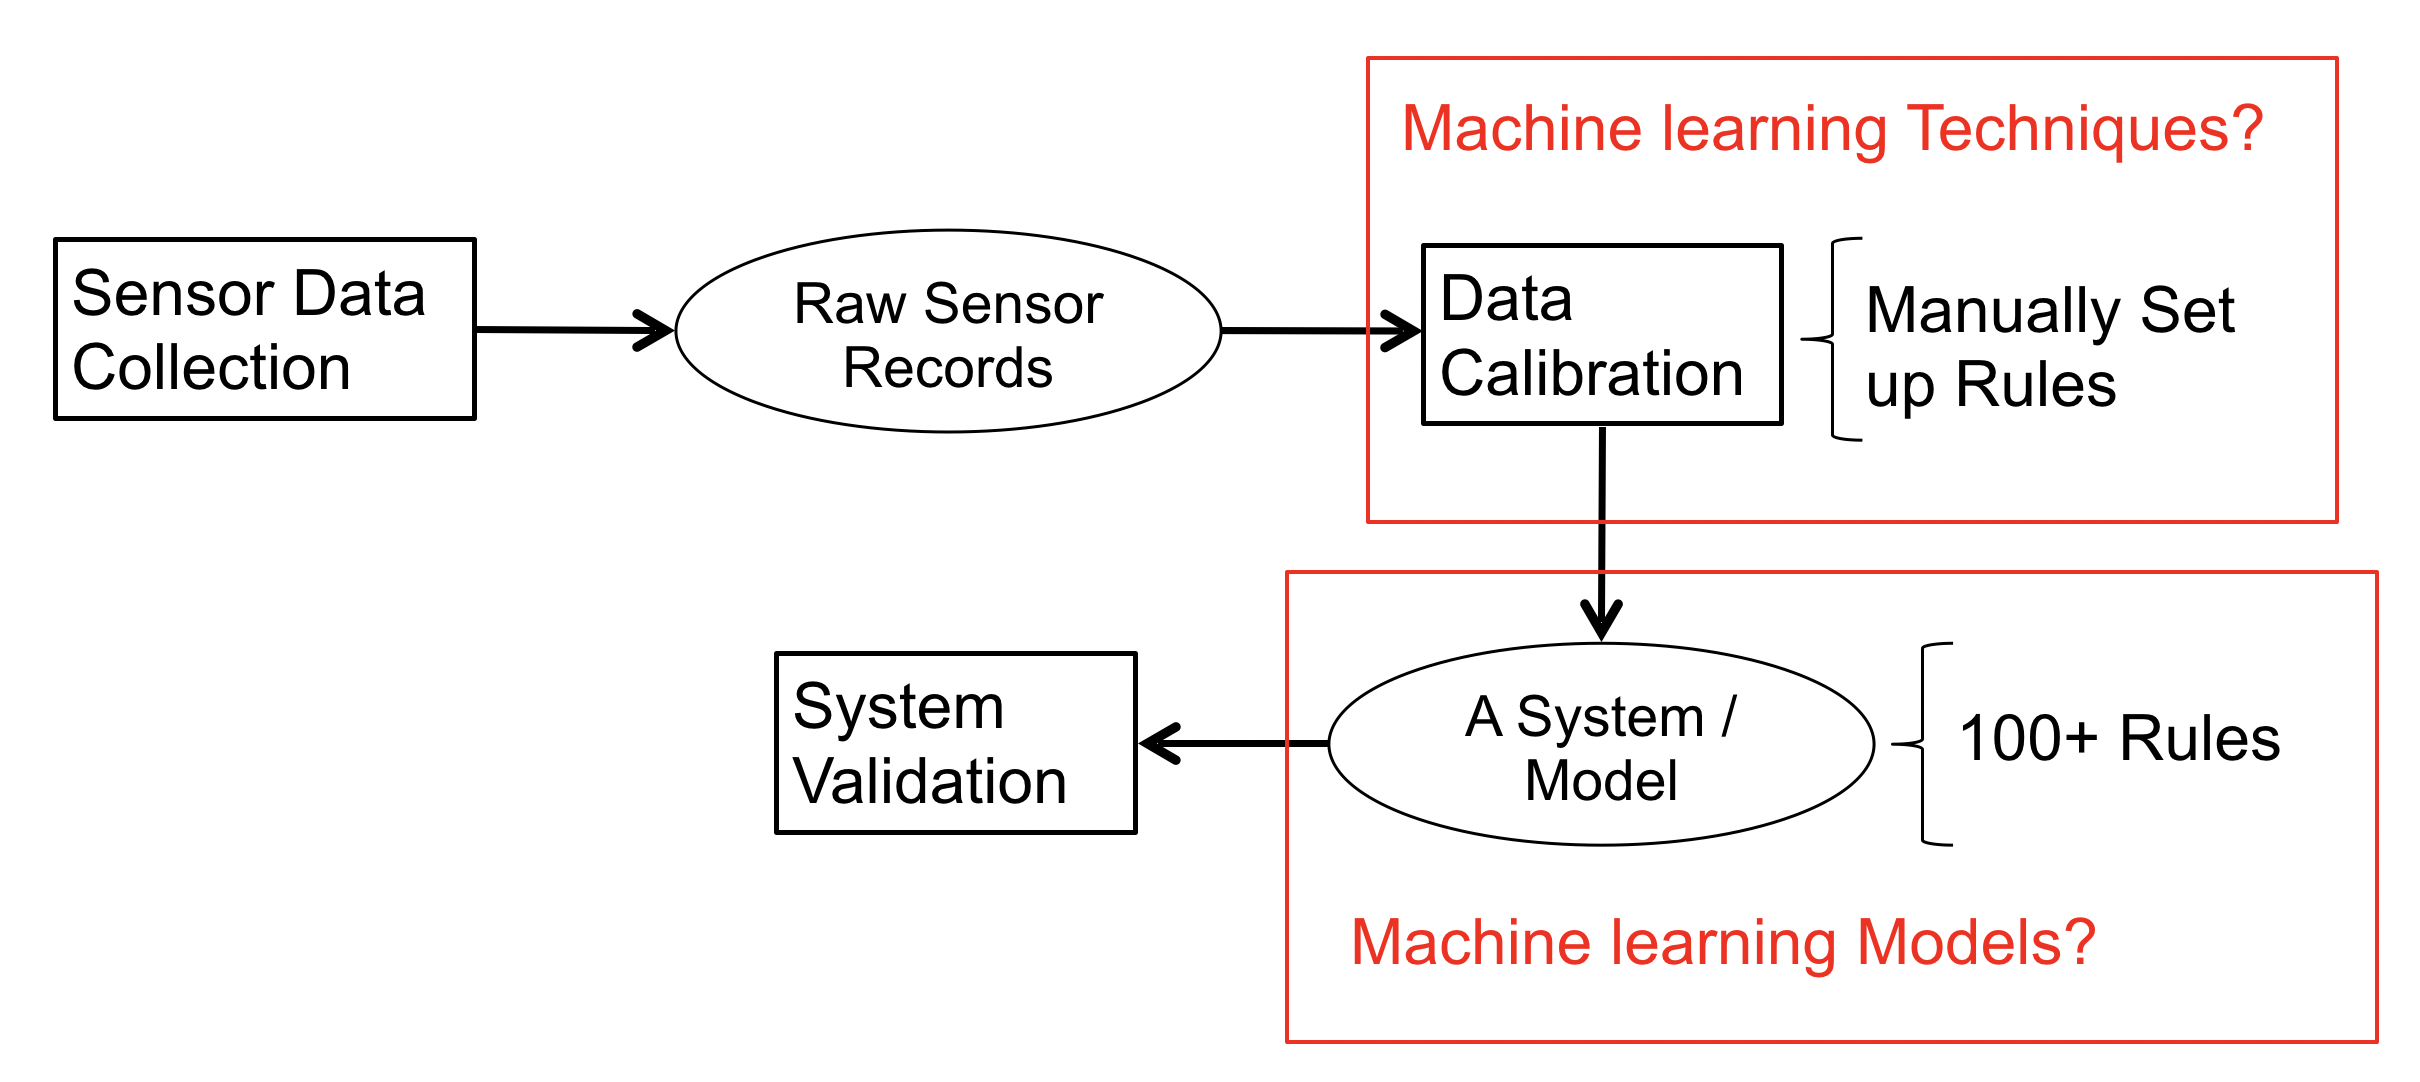
\includegraphics[width=0.75\textwidth]{related_work.png}
	\caption{The-State-of-the-Art Strategy of Blip Systems A/S}
	\label{fig:strategy_of_blip}
\end{figure}

\par
This project focuses on exploring machine learning techniques to distinguish and classify the raw sensor data of mobile devices. We should provide a more efficient solution for data calibration and modelling without the need for fine-grained manually created logic. Rather than analysing the data of the entire airport, a specific area - the arrival gate - was chosen.\newline

\par
The involved data set is a set of measurements collected from the sensors placed throughout the area. The raw, multidimensional data comes with intricacies of wireless signals and mobile device, such as variance in signal strength or edge cases create by different device usage patterns. This poses a significant challenge for data processing, which is why the data will need to be modelled to both represent the behaviour of passengers appropriately, as well as conform to the constraints of machine learning techniques to be utilised. \newline

\par
To achieve the goal of this project, the following methods will be used:

We will conduct our initial experiments using Label propagation as a baseline method with the focus on modelling the similarities among data in form of multivariate times series. The baseline will serve us as a simple method to get some initial results and help us to better understand the data, as well as to decide on further direction.
Afterwards, we will experiment with Decision Trees, a feature-centric technique, which will demand features to be extracted from the data (feature engineering).
Finally, the last stage will require a more complex, deep learning model such as Convolutional Neural Networks, where the objective will be to discover and learn patterns in the data automatically.

%\input{Report/probAnalysis.tex}


\clearpage

%\pagenumbering{gobble}

%Figurliste
\listoffigures

%Tabelliste
\listoftables

%Litteraturliste
\bibliography{literature}

%Bilag___APENDICE
%\input{Bilag/bilag.tex}
	
\end{document}
